
\documentclass{article} % For LaTeX2e
\usepackage{iclr2021_conference,times}

% Optional math commands from https://github.com/goodfeli/dlbook_notation.
%%%%% NEW MATH DEFINITIONS %%%%%

\usepackage{amsmath,amsfonts,bm}

% Mark sections of captions for referring to divisions of figures
\newcommand{\figleft}{{\em (Left)}}
\newcommand{\figcenter}{{\em (Center)}}
\newcommand{\figright}{{\em (Right)}}
\newcommand{\figtop}{{\em (Top)}}
\newcommand{\figbottom}{{\em (Bottom)}}
\newcommand{\captiona}{{\em (a)}}
\newcommand{\captionb}{{\em (b)}}
\newcommand{\captionc}{{\em (c)}}
\newcommand{\captiond}{{\em (d)}}

% Highlight a newly defined term
\newcommand{\newterm}[1]{{\bf #1}}


% Figure reference, lower-case.
\def\figref#1{figure~\ref{#1}}
% Figure reference, capital. For start of sentence
\def\Figref#1{Figure~\ref{#1}}
\def\twofigref#1#2{figures \ref{#1} and \ref{#2}}
\def\quadfigref#1#2#3#4{figures \ref{#1}, \ref{#2}, \ref{#3} and \ref{#4}}
% Section reference, lower-case.
\def\secref#1{section~\ref{#1}}
% Section reference, capital.
\def\Secref#1{Section~\ref{#1}}
% Reference to two sections.
\def\twosecrefs#1#2{sections \ref{#1} and \ref{#2}}
% Reference to three sections.
\def\secrefs#1#2#3{sections \ref{#1}, \ref{#2} and \ref{#3}}
% Reference to an equation, lower-case.
\def\eqref#1{equation~\ref{#1}}
% Reference to an equation, upper case
\def\Eqref#1{Equation~\ref{#1}}
% A raw reference to an equation---avoid using if possible
\def\plaineqref#1{\ref{#1}}
% Reference to a chapter, lower-case.
\def\chapref#1{chapter~\ref{#1}}
% Reference to an equation, upper case.
\def\Chapref#1{Chapter~\ref{#1}}
% Reference to a range of chapters
\def\rangechapref#1#2{chapters\ref{#1}--\ref{#2}}
% Reference to an algorithm, lower-case.
\def\algref#1{algorithm~\ref{#1}}
% Reference to an algorithm, upper case.
\def\Algref#1{Algorithm~\ref{#1}}
\def\twoalgref#1#2{algorithms \ref{#1} and \ref{#2}}
\def\Twoalgref#1#2{Algorithms \ref{#1} and \ref{#2}}
% Reference to a part, lower case
\def\partref#1{part~\ref{#1}}
% Reference to a part, upper case
\def\Partref#1{Part~\ref{#1}}
\def\twopartref#1#2{parts \ref{#1} and \ref{#2}}

\def\ceil#1{\lceil #1 \rceil}
\def\floor#1{\lfloor #1 \rfloor}
\def\1{\bm{1}}
\newcommand{\train}{\mathcal{D}}
\newcommand{\valid}{\mathcal{D_{\mathrm{valid}}}}
\newcommand{\test}{\mathcal{D_{\mathrm{test}}}}

\def\eps{{\epsilon}}


% Random variables
\def\reta{{\textnormal{$\eta$}}}
\def\ra{{\textnormal{a}}}
\def\rb{{\textnormal{b}}}
\def\rc{{\textnormal{c}}}
\def\rd{{\textnormal{d}}}
\def\re{{\textnormal{e}}}
\def\rf{{\textnormal{f}}}
\def\rg{{\textnormal{g}}}
\def\rh{{\textnormal{h}}}
\def\ri{{\textnormal{i}}}
\def\rj{{\textnormal{j}}}
\def\rk{{\textnormal{k}}}
\def\rl{{\textnormal{l}}}
% rm is already a command, just don't name any random variables m
\def\rn{{\textnormal{n}}}
\def\ro{{\textnormal{o}}}
\def\rp{{\textnormal{p}}}
\def\rq{{\textnormal{q}}}
\def\rr{{\textnormal{r}}}
\def\rs{{\textnormal{s}}}
\def\rt{{\textnormal{t}}}
\def\ru{{\textnormal{u}}}
\def\rv{{\textnormal{v}}}
\def\rw{{\textnormal{w}}}
\def\rx{{\textnormal{x}}}
\def\ry{{\textnormal{y}}}
\def\rz{{\textnormal{z}}}

% Random vectors
\def\rvepsilon{{\mathbf{\epsilon}}}
\def\rvtheta{{\mathbf{\theta}}}
\def\rva{{\mathbf{a}}}
\def\rvb{{\mathbf{b}}}
\def\rvc{{\mathbf{c}}}
\def\rvd{{\mathbf{d}}}
\def\rve{{\mathbf{e}}}
\def\rvf{{\mathbf{f}}}
\def\rvg{{\mathbf{g}}}
\def\rvh{{\mathbf{h}}}
\def\rvu{{\mathbf{i}}}
\def\rvj{{\mathbf{j}}}
\def\rvk{{\mathbf{k}}}
\def\rvl{{\mathbf{l}}}
\def\rvm{{\mathbf{m}}}
\def\rvn{{\mathbf{n}}}
\def\rvo{{\mathbf{o}}}
\def\rvp{{\mathbf{p}}}
\def\rvq{{\mathbf{q}}}
\def\rvr{{\mathbf{r}}}
\def\rvs{{\mathbf{s}}}
\def\rvt{{\mathbf{t}}}
\def\rvu{{\mathbf{u}}}
\def\rvv{{\mathbf{v}}}
\def\rvw{{\mathbf{w}}}
\def\rvx{{\mathbf{x}}}
\def\rvy{{\mathbf{y}}}
\def\rvz{{\mathbf{z}}}

% Elements of random vectors
\def\erva{{\textnormal{a}}}
\def\ervb{{\textnormal{b}}}
\def\ervc{{\textnormal{c}}}
\def\ervd{{\textnormal{d}}}
\def\erve{{\textnormal{e}}}
\def\ervf{{\textnormal{f}}}
\def\ervg{{\textnormal{g}}}
\def\ervh{{\textnormal{h}}}
\def\ervi{{\textnormal{i}}}
\def\ervj{{\textnormal{j}}}
\def\ervk{{\textnormal{k}}}
\def\ervl{{\textnormal{l}}}
\def\ervm{{\textnormal{m}}}
\def\ervn{{\textnormal{n}}}
\def\ervo{{\textnormal{o}}}
\def\ervp{{\textnormal{p}}}
\def\ervq{{\textnormal{q}}}
\def\ervr{{\textnormal{r}}}
\def\ervs{{\textnormal{s}}}
\def\ervt{{\textnormal{t}}}
\def\ervu{{\textnormal{u}}}
\def\ervv{{\textnormal{v}}}
\def\ervw{{\textnormal{w}}}
\def\ervx{{\textnormal{x}}}
\def\ervy{{\textnormal{y}}}
\def\ervz{{\textnormal{z}}}

% Random matrices
\def\rmA{{\mathbf{A}}}
\def\rmB{{\mathbf{B}}}
\def\rmC{{\mathbf{C}}}
\def\rmD{{\mathbf{D}}}
\def\rmE{{\mathbf{E}}}
\def\rmF{{\mathbf{F}}}
\def\rmG{{\mathbf{G}}}
\def\rmH{{\mathbf{H}}}
\def\rmI{{\mathbf{I}}}
\def\rmJ{{\mathbf{J}}}
\def\rmK{{\mathbf{K}}}
\def\rmL{{\mathbf{L}}}
\def\rmM{{\mathbf{M}}}
\def\rmN{{\mathbf{N}}}
\def\rmO{{\mathbf{O}}}
\def\rmP{{\mathbf{P}}}
\def\rmQ{{\mathbf{Q}}}
\def\rmR{{\mathbf{R}}}
\def\rmS{{\mathbf{S}}}
\def\rmT{{\mathbf{T}}}
\def\rmU{{\mathbf{U}}}
\def\rmV{{\mathbf{V}}}
\def\rmW{{\mathbf{W}}}
\def\rmX{{\mathbf{X}}}
\def\rmY{{\mathbf{Y}}}
\def\rmZ{{\mathbf{Z}}}

% Elements of random matrices
\def\ermA{{\textnormal{A}}}
\def\ermB{{\textnormal{B}}}
\def\ermC{{\textnormal{C}}}
\def\ermD{{\textnormal{D}}}
\def\ermE{{\textnormal{E}}}
\def\ermF{{\textnormal{F}}}
\def\ermG{{\textnormal{G}}}
\def\ermH{{\textnormal{H}}}
\def\ermI{{\textnormal{I}}}
\def\ermJ{{\textnormal{J}}}
\def\ermK{{\textnormal{K}}}
\def\ermL{{\textnormal{L}}}
\def\ermM{{\textnormal{M}}}
\def\ermN{{\textnormal{N}}}
\def\ermO{{\textnormal{O}}}
\def\ermP{{\textnormal{P}}}
\def\ermQ{{\textnormal{Q}}}
\def\ermR{{\textnormal{R}}}
\def\ermS{{\textnormal{S}}}
\def\ermT{{\textnormal{T}}}
\def\ermU{{\textnormal{U}}}
\def\ermV{{\textnormal{V}}}
\def\ermW{{\textnormal{W}}}
\def\ermX{{\textnormal{X}}}
\def\ermY{{\textnormal{Y}}}
\def\ermZ{{\textnormal{Z}}}

% Vectors
\def\vzero{{\bm{0}}}
\def\vone{{\bm{1}}}
\def\vmu{{\bm{\mu}}}
\def\vtheta{{\bm{\theta}}}
\def\va{{\bm{a}}}
\def\vb{{\bm{b}}}
\def\vc{{\bm{c}}}
\def\vd{{\bm{d}}}
\def\ve{{\bm{e}}}
\def\vf{{\bm{f}}}
\def\vg{{\bm{g}}}
\def\vh{{\bm{h}}}
\def\vi{{\bm{i}}}
\def\vj{{\bm{j}}}
\def\vk{{\bm{k}}}
\def\vl{{\bm{l}}}
\def\vm{{\bm{m}}}
\def\vn{{\bm{n}}}
\def\vo{{\bm{o}}}
\def\vp{{\bm{p}}}
\def\vq{{\bm{q}}}
\def\vr{{\bm{r}}}
\def\vs{{\bm{s}}}
\def\vt{{\bm{t}}}
\def\vu{{\bm{u}}}
\def\vv{{\bm{v}}}
\def\vw{{\bm{w}}}
\def\vx{{\bm{x}}}
\def\vy{{\bm{y}}}
\def\vz{{\bm{z}}}

% Elements of vectors
\def\evalpha{{\alpha}}
\def\evbeta{{\beta}}
\def\evepsilon{{\epsilon}}
\def\evlambda{{\lambda}}
\def\evomega{{\omega}}
\def\evmu{{\mu}}
\def\evpsi{{\psi}}
\def\evsigma{{\sigma}}
\def\evtheta{{\theta}}
\def\eva{{a}}
\def\evb{{b}}
\def\evc{{c}}
\def\evd{{d}}
\def\eve{{e}}
\def\evf{{f}}
\def\evg{{g}}
\def\evh{{h}}
\def\evi{{i}}
\def\evj{{j}}
\def\evk{{k}}
\def\evl{{l}}
\def\evm{{m}}
\def\evn{{n}}
\def\evo{{o}}
\def\evp{{p}}
\def\evq{{q}}
\def\evr{{r}}
\def\evs{{s}}
\def\evt{{t}}
\def\evu{{u}}
\def\evv{{v}}
\def\evw{{w}}
\def\evx{{x}}
\def\evy{{y}}
\def\evz{{z}}

% Matrix
\def\mA{{\bm{A}}}
\def\mB{{\bm{B}}}
\def\mC{{\bm{C}}}
\def\mD{{\bm{D}}}
\def\mE{{\bm{E}}}
\def\mF{{\bm{F}}}
\def\mG{{\bm{G}}}
\def\mH{{\bm{H}}}
\def\mI{{\bm{I}}}
\def\mJ{{\bm{J}}}
\def\mK{{\bm{K}}}
\def\mL{{\bm{L}}}
\def\mM{{\bm{M}}}
\def\mN{{\bm{N}}}
\def\mO{{\bm{O}}}
\def\mP{{\bm{P}}}
\def\mQ{{\bm{Q}}}
\def\mR{{\bm{R}}}
\def\mS{{\bm{S}}}
\def\mT{{\bm{T}}}
\def\mU{{\bm{U}}}
\def\mV{{\bm{V}}}
\def\mW{{\bm{W}}}
\def\mX{{\bm{X}}}
\def\mY{{\bm{Y}}}
\def\mZ{{\bm{Z}}}
\def\mBeta{{\bm{\beta}}}
\def\mPhi{{\bm{\Phi}}}
\def\mLambda{{\bm{\Lambda}}}
\def\mSigma{{\bm{\Sigma}}}

% Tensor
\DeclareMathAlphabet{\mathsfit}{\encodingdefault}{\sfdefault}{m}{sl}
\SetMathAlphabet{\mathsfit}{bold}{\encodingdefault}{\sfdefault}{bx}{n}
\newcommand{\tens}[1]{\bm{\mathsfit{#1}}}
\def\tA{{\tens{A}}}
\def\tB{{\tens{B}}}
\def\tC{{\tens{C}}}
\def\tD{{\tens{D}}}
\def\tE{{\tens{E}}}
\def\tF{{\tens{F}}}
\def\tG{{\tens{G}}}
\def\tH{{\tens{H}}}
\def\tI{{\tens{I}}}
\def\tJ{{\tens{J}}}
\def\tK{{\tens{K}}}
\def\tL{{\tens{L}}}
\def\tM{{\tens{M}}}
\def\tN{{\tens{N}}}
\def\tO{{\tens{O}}}
\def\tP{{\tens{P}}}
\def\tQ{{\tens{Q}}}
\def\tR{{\tens{R}}}
\def\tS{{\tens{S}}}
\def\tT{{\tens{T}}}
\def\tU{{\tens{U}}}
\def\tV{{\tens{V}}}
\def\tW{{\tens{W}}}
\def\tX{{\tens{X}}}
\def\tY{{\tens{Y}}}
\def\tZ{{\tens{Z}}}


% Graph
\def\gA{{\mathcal{A}}}
\def\gB{{\mathcal{B}}}
\def\gC{{\mathcal{C}}}
\def\gD{{\mathcal{D}}}
\def\gE{{\mathcal{E}}}
\def\gF{{\mathcal{F}}}
\def\gG{{\mathcal{G}}}
\def\gH{{\mathcal{H}}}
\def\gI{{\mathcal{I}}}
\def\gJ{{\mathcal{J}}}
\def\gK{{\mathcal{K}}}
\def\gL{{\mathcal{L}}}
\def\gM{{\mathcal{M}}}
\def\gN{{\mathcal{N}}}
\def\gO{{\mathcal{O}}}
\def\gP{{\mathcal{P}}}
\def\gQ{{\mathcal{Q}}}
\def\gR{{\mathcal{R}}}
\def\gS{{\mathcal{S}}}
\def\gT{{\mathcal{T}}}
\def\gU{{\mathcal{U}}}
\def\gV{{\mathcal{V}}}
\def\gW{{\mathcal{W}}}
\def\gX{{\mathcal{X}}}
\def\gY{{\mathcal{Y}}}
\def\gZ{{\mathcal{Z}}}

% Sets
\def\sA{{\mathbb{A}}}
\def\sB{{\mathbb{B}}}
\def\sC{{\mathbb{C}}}
\def\sD{{\mathbb{D}}}
% Don't use a set called E, because this would be the same as our symbol
% for expectation.
\def\sF{{\mathbb{F}}}
\def\sG{{\mathbb{G}}}
\def\sH{{\mathbb{H}}}
\def\sI{{\mathbb{I}}}
\def\sJ{{\mathbb{J}}}
\def\sK{{\mathbb{K}}}
\def\sL{{\mathbb{L}}}
\def\sM{{\mathbb{M}}}
\def\sN{{\mathbb{N}}}
\def\sO{{\mathbb{O}}}
\def\sP{{\mathbb{P}}}
\def\sQ{{\mathbb{Q}}}
\def\sR{{\mathbb{R}}}
\def\sS{{\mathbb{S}}}
\def\sT{{\mathbb{T}}}
\def\sU{{\mathbb{U}}}
\def\sV{{\mathbb{V}}}
\def\sW{{\mathbb{W}}}
\def\sX{{\mathbb{X}}}
\def\sY{{\mathbb{Y}}}
\def\sZ{{\mathbb{Z}}}

% Entries of a matrix
\def\emLambda{{\Lambda}}
\def\emA{{A}}
\def\emB{{B}}
\def\emC{{C}}
\def\emD{{D}}
\def\emE{{E}}
\def\emF{{F}}
\def\emG{{G}}
\def\emH{{H}}
\def\emI{{I}}
\def\emJ{{J}}
\def\emK{{K}}
\def\emL{{L}}
\def\emM{{M}}
\def\emN{{N}}
\def\emO{{O}}
\def\emP{{P}}
\def\emQ{{Q}}
\def\emR{{R}}
\def\emS{{S}}
\def\emT{{T}}
\def\emU{{U}}
\def\emV{{V}}
\def\emW{{W}}
\def\emX{{X}}
\def\emY{{Y}}
\def\emZ{{Z}}
\def\emSigma{{\Sigma}}

% entries of a tensor
% Same font as tensor, without \bm wrapper
\newcommand{\etens}[1]{\mathsfit{#1}}
\def\etLambda{{\etens{\Lambda}}}
\def\etA{{\etens{A}}}
\def\etB{{\etens{B}}}
\def\etC{{\etens{C}}}
\def\etD{{\etens{D}}}
\def\etE{{\etens{E}}}
\def\etF{{\etens{F}}}
\def\etG{{\etens{G}}}
\def\etH{{\etens{H}}}
\def\etI{{\etens{I}}}
\def\etJ{{\etens{J}}}
\def\etK{{\etens{K}}}
\def\etL{{\etens{L}}}
\def\etM{{\etens{M}}}
\def\etN{{\etens{N}}}
\def\etO{{\etens{O}}}
\def\etP{{\etens{P}}}
\def\etQ{{\etens{Q}}}
\def\etR{{\etens{R}}}
\def\etS{{\etens{S}}}
\def\etT{{\etens{T}}}
\def\etU{{\etens{U}}}
\def\etV{{\etens{V}}}
\def\etW{{\etens{W}}}
\def\etX{{\etens{X}}}
\def\etY{{\etens{Y}}}
\def\etZ{{\etens{Z}}}

% The true underlying data generating distribution
\newcommand{\pdata}{p_{\rm{data}}}
% The empirical distribution defined by the training set
\newcommand{\ptrain}{\hat{p}_{\rm{data}}}
\newcommand{\Ptrain}{\hat{P}_{\rm{data}}}
% The model distribution
\newcommand{\pmodel}{p_{\rm{model}}}
\newcommand{\Pmodel}{P_{\rm{model}}}
\newcommand{\ptildemodel}{\tilde{p}_{\rm{model}}}
% Stochastic autoencoder distributions
\newcommand{\pencode}{p_{\rm{encoder}}}
\newcommand{\pdecode}{p_{\rm{decoder}}}
\newcommand{\precons}{p_{\rm{reconstruct}}}

\newcommand{\laplace}{\mathrm{Laplace}} % Laplace distribution

\newcommand{\E}{\mathbb{E}}
\newcommand{\Ls}{\mathcal{L}}
\newcommand{\R}{\mathbb{R}}
\newcommand{\emp}{\tilde{p}}
\newcommand{\lr}{\alpha}
\newcommand{\reg}{\lambda}
\newcommand{\rect}{\mathrm{rectifier}}
\newcommand{\softmax}{\mathrm{softmax}}
\newcommand{\sigmoid}{\sigma}
\newcommand{\softplus}{\zeta}
\newcommand{\KL}{D_{\mathrm{KL}}}
\newcommand{\Var}{\mathrm{Var}}
\newcommand{\standarderror}{\mathrm{SE}}
\newcommand{\Cov}{\mathrm{Cov}}
% Wolfram Mathworld says $L^2$ is for function spaces and $\ell^2$ is for vectors
% But then they seem to use $L^2$ for vectors throughout the site, and so does
% wikipedia.
\newcommand{\normlzero}{L^0}
\newcommand{\normlone}{L^1}
\newcommand{\normltwo}{L^2}
\newcommand{\normlp}{L^p}
\newcommand{\normmax}{L^\infty}

\newcommand{\parents}{Pa} % See usage in notation.tex. Chosen to match Daphne's book.

\DeclareMathOperator*{\argmax}{arg\,max}
\DeclareMathOperator*{\argmin}{arg\,min}

\DeclareMathOperator{\sign}{sign}
\DeclareMathOperator{\Tr}{Tr}
\let\ab\allowbreak


\usepackage{hyperref}
\usepackage{url}

\usepackage{algorithm}
\usepackage{algorithmicx}
\usepackage{algpseudocode}
\usepackage{amsmath}
\usepackage{caption}
\usepackage{graphicx}
\usepackage{subfigure}

\title{Multi-agent exploration through Intrinsic Motivation Credit Assignment}

% Authors must not appear in the submitted version. They should be hidden
% as long as the \iclrfinalcopy macro remains commented out below.
% Non-anonymous submissions will be rejected without review.

\iffalse
\author{Antiquus S.~Hippocampus, Natalia Cerebro \& Amelie P. Amygdale \thanks{ Use footnote for providing further information
about author (webpage, alternative address)---\emph{not} for acknowledging
funding agencies.  Funding acknowledgements go at the end of the paper.} \\
Department of Computer Science\\
Cranberry-Lemon University\\
Pittsburgh, PA 15213, USA \\
\texttt{\{hippo,brain,jen\}@cs.cranberry-lemon.edu} \\
\And
Ji Q. Ren \& Yevgeny LeNet \\
Department of Computational Neuroscience \\
University of the Witwatersrand \\
Joburg, South Africa \\
\texttt{\{robot,net\}@wits.ac.za} \\
\AND
Coauthor \\
Affiliation \\
Address \\
\texttt{email}
}
\fi

% The \author macro works with any number of authors. There are two commands
% used to separate the names and addresses of multiple authors: \And and \AND.
%
% Using \And between authors leaves it to \LaTeX{} to determine where to break
% the lines. Using \AND forces a linebreak at that point. So, if \LaTeX{}
% puts 3 of 4 authors names on the first line, and the last on the second
% line, try using \AND instead of \And before the third author name.

\newcommand{\fix}{\marginpar{FIX}}
\newcommand{\new}{\marginpar{NEW}}

%\iclrfinalcopy % Uncomment for camera-ready version, but NOT for submission.
\begin{document}


\maketitle

\begin{abstract}
Sparse rewards are common in real-world environment, which brings challenges to reinforcement learning, previous works have made great progress in single-agent domain by introducing intrinsic rewards to encourage agent to access relatively new states in their state space, directly applying these methods to multi-agent setting results in agents exploring independently. In this work we attempt to designing intrinsic rewards for individual agent in order to provide more accurate exploration guidance for them. Concretely, we propose Intrinsic-Motivation-Credit-Assignment, a novel mechanism which derive exploration bonus for each agent according to their contribution to the whole system's exploration tendency, which measured by global intrinsic rewards. We verify the effectiveness of our mechanism on three cooperate exploration tasks, for each task we choose different exploration algorithm according to its feature including count-based algorithm, random network distillation and successor feature control. Results show that these algorithms greatly improved their performance with our mechanism in exploration-challenging tasks.  
\end{abstract}

\section{Introduction}

Reinforcement learning algorithm has achieve excellent performance in many scenarios, such as Atari games\cite{Human-level}, the board game Go\cite{Go}, and simulated robotic continuous control\cite{continuous}, the goal is to learn a policy to maximizes the accumulative reward during agent interacting with the environment. Most of reinforcement learning algorithm's success depend on frequent reward signals from environment, which known as dense rewards, such as expert-designed rewards\cite{expert}, distance to the goal\cite{distance} or the games' scores\cite{Human-level}, however, those algorithm often struggle in real-world sparse rewards scenarios, where agent only receive reward signal when accomplish whole task. A widely used method proposed to address the sparse reward issue is using intrinsic motivation as an exploration bias to guide agent to explore unseen region. Many previous works have achieved satisfactory performance by adopting intrinsic reward as exploration bonus, however, most of them focus on single agent setting\cite{Count,ICM,SF,RND,RIDE,NGU}, the literature on multi-agent is relatively scarce\cite{Influence,Social,Synergistic,Cooperative}. Since intrinsic rewards are extra learning signal, it may destabilize the learning objective if it accounts too much of the overall rewards or it can not help improving exploration ability of agent if accounts too little, this make multi-agent exploration using intrinsic rewards especially difficult as each agent's exploration bonus need to be carefully designed. This paper aims to take a step towards this goal, we study how to manipulate individual intrinsic rewards as a more accurate exploration guidance for each agent, training with these extra rewards can help a group of agents explore their state space cooperatively.

We propose Intrinsic-Motivation-Credit-Assignment, a novel algorithm which derive exploration bonus for each agent according to their contribution to the whole system’s exploration tendency which measured by global intrinsic rewards, IMCA

Credit assignment is another crucial challenge in multi-agent reinforcement learning:in most multi-agent cooperative tasks, agents' joint actions typically generate only global rewards, making it difficult for each agent to deduce its own contribution to the team's success. Previous work using counterfactual baseline like COMA\cite{COMA} to estimate advantage function for updating each agent's policy, or decomposed the central state-action value function to get individual value function of each agent and achieve satisfactory performance\cite{VDN,QMIX}. All value networks used in those work are trained with extrinsic reward from environment, none of them consider credit assignment problem in intrinsic rewards. Our motivation is that intrinsic rewards as reward signals have the same shortcoming when applying to training process, i.e., credit assignment, agents trained with same intrinsic rewards are motivated equally, however, their contributions to the overall intrinsic rewards received are different, we take a example to illustrate this issue, as shown in \ref{motivation1}, two agents, i.e., agent$1$ and agent $2$ are required to search the big room with two small rooms, i.e., room$A$ and room$B$, suppose that agent$1$ is familiar with room$A$ and agent$2$ is not familiar with room$B$ , that means agent$1$ step into room$A$ multiple times, and agent$2$ rarely enter room$B$, more formally, mark the state-action pairs of agent$1$ and agent$2$ at current time shown in figure[] as $\left(o_{1}, a_{1}\right)$ and $\left(o_{2}, a_{2}\right)$ respectively, and joint state-action pair as $(S, U)$, where $S=\left\langle o_{1}, o_{2}\right\rangle$ and $U=\left\langle a_{1}, a_{2}\right\rangle$, the joint state-action novelty of $(S, U)$ is very high mainly due to agent$2$ rarely take action $a_{2}$ at state $o_{2}$, although we can design high novelty based intrinsic rewards equally for agent$1$ and agent$2$, it is more reasonable to distinguish them by their contribution, that is intrinsically motivated agent$2$ more to visit room$B$ while less for agent$1$. One may have doubt why not let agent$1$ and agent$2$ explore their state space independently, we take another example to illustrate the irrationality of independent exploration, as shown in \ref{motivation2}, as the same situation as \ref{motivation1}, the two agents are required to complete the task cooperatively, i.e., press the buttons(green squares) concurrently, in this task, independent exploration is not suitable because agent$1$ may rarely enter the room$A$ in the later stage duo to fewer exploration bonus, which leads to the rare occurrence of joint state-action pair $(S, U)$, thus they need a exploration strategy which motivate the system to explore all novel joint state-action space.

In addition, note the coordinated nature of multi-agent cooperative tasks, a team of homogeneous agents explore their joint state space cooperatively should take into account the permutation invariance of their position, otherwise may leads to redundant explore actions. For example, the relative locations of $n$ homogeneous agents can be represented as $n!$ different states, when focusing on the relative configuration among agents, n! different states represent the same state, we use a example to illustrate it, as shown in \ref{motivation3}, compared with figure[1], agent$1$ and agent$2$ exchange their positions, i.e., agent$1$ and agent$2$ are about to entering the room$B$ and room$B$ respectively, since the two agents are homogeneous, they search the same space from the perspective of whole task, thus the two situations should be treated equally, in another word, agents should be motivated equally using intrinsic rewards.

we claim the irrationality when directly extend single-agent algorithm to multi-agent system, and proposed an Intrinsic-Motivation-Credit-Assignment mechanism, with this mechanism, a group of agents show stronger exploration ability and perform better in cooperative exploration tasks. Also, our mechanism can be easily combined with existing algorithm, we verify the effectiveness of our mechanism using PPO as basic algorithm.

\begin{figure}
\centering
    \subfigure[] {
     \label{motivation1}
     \begin{minipage}[t]{0.3\linewidth}
     \centering
     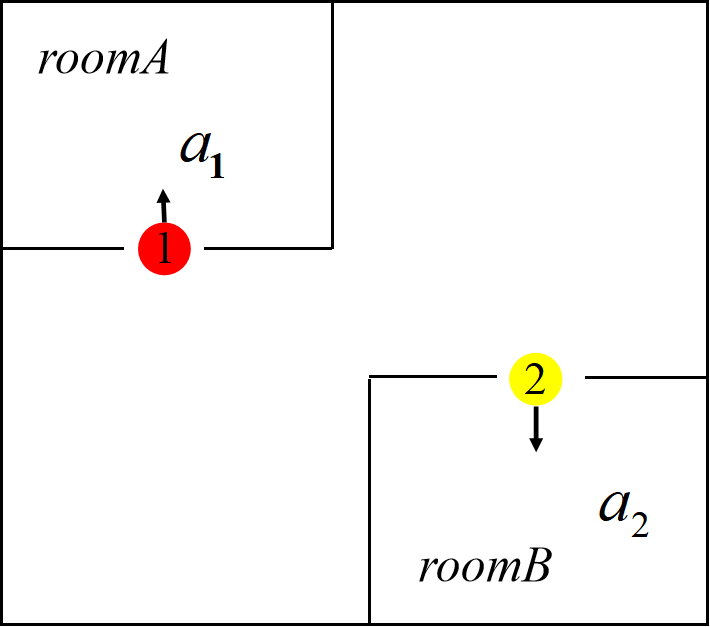
\includegraphics[width=1.5in]{picture/motivation1.png}  
     \end{minipage}
    }
    \subfigure[] {
     \label{motivation2}     
     \begin{minipage}[t]{0.3\linewidth}
     \centering
     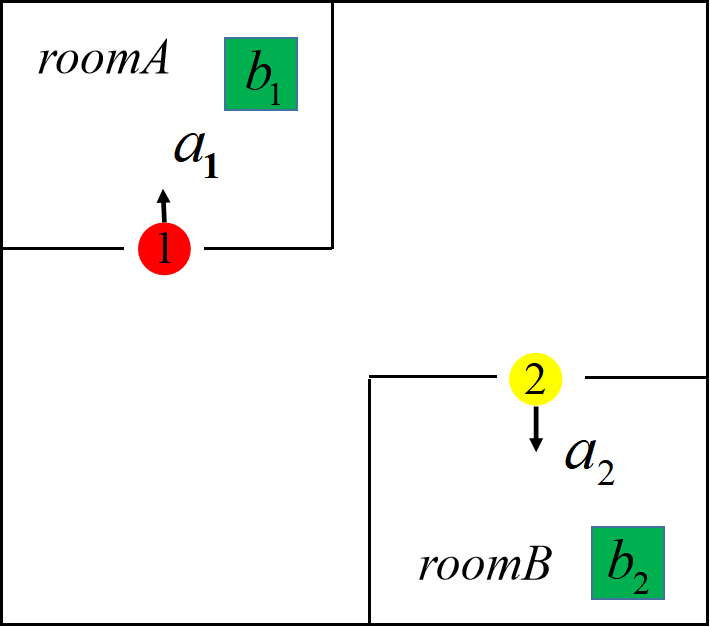
\includegraphics[width=1.5in]{picture/motivation2.png}
     \end{minipage}
    } 
    \subfigure[] {
     \label{motivation3}
     \begin{minipage}[t]{0.3\linewidth}
     \centering
     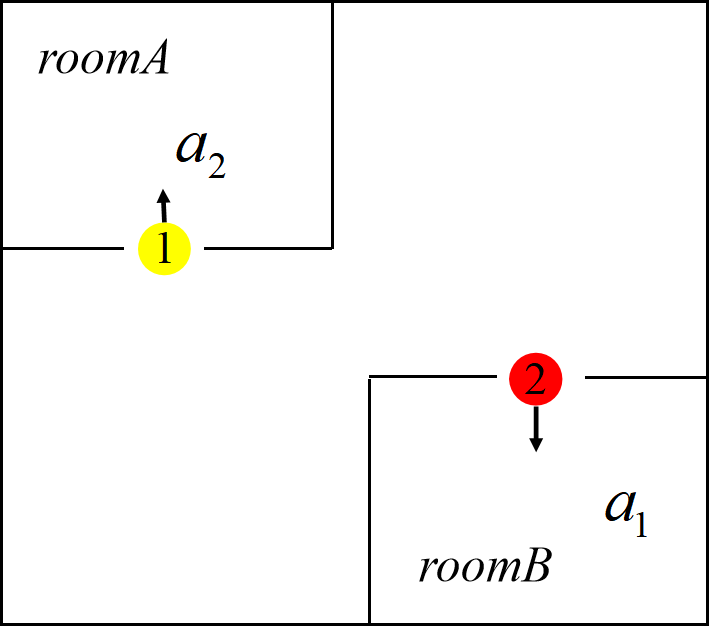
\includegraphics[width=1.5in]{picture/motivation3.png}
     \end{minipage}
    }
    \caption{search grid}
    \label{motivation}
\end{figure}

\section{Related work}
\subsection{Intrinsic Motivation for Single-Agent Exploration}
To overcome sparse reward challenge in real-world scenarios, researchers have long worked on improving exploration in reinforcement learning. One commonly used way is adding intrinsic reward as exploration bonus to encourage agent to visit novel state, a variety of methods were proposed for designing such intrinsic reward, [] use inverse state-action counts in tabular setting[], [] scale those count-based approach to large state space using pseudo state counts, [ICM] trained a model for predicting next state and use predict error as exploration bonus to guide the agent to explore what makes it curious, [RND] use random state embedding network distillation error to define novelty of a state, [SF] calculate distance between successor feature of two consecutive states as exploration bonus while [] use the distance between the learned state representations. 

\subsection{Multi-agent Exploration}
Compare to single agent, exploration is more difficult in multi-agent domain considering the unique cooperative property. [load balancing] study exploration of a large joint action space toward handle a load balancing problem, [coordinate exploration] design several intrinsic reward type and dynamically select one of them per episode to train, [social influence] define an intrinsic reward function based on influence on other agents' actions, which encourages agents to take actions have the biggest effect on other agents’ behavior, [influence based] measures the influence of one agent on other agent's transition function (EITI) and rewarding structure(EDTI) and use the mutual information as a regularizer to the learning objective. Some of the above approach use novelty based intrinsic reward as a baseline but none of them consider the 

\subsection{Multi-Agent Credit Assignment under centralize learning with decentralise execution paradigm}
Centralised learning with fully decentralised execution is well adopted in multi-agent learning [MADDPG, COMA], agents have access to global information during the training phase while only act upon their own observations during execution phase, in cooperative tasks they always awarded together as a team, however, the global reward received from the environment can't distinguish the contribution of each agent to the team's success, making it difficult to train their local policy. Many previous works have proposed approaches to address 
this issue and have obtained empirically solid results. [COMA] estimate a counterfactual advantage function for each agent to identify the real advantage of current action compared with other actions, [VDN] decomposed a central state-action value function into a sum of individual agent terms while [Qix] let the global value function be monotonic with each agent's value function. 

\section{background}
\subsection{Dec-POMDP}
In this work, we restrict ourselves to multi-agent fully cooperative tasks, which is modeled as a decentralized POMDP(Dec-POMDP). A Dec-POMDP is defined as a tuple $\left\langle\mathcal{S},U, P, r,O,\mathcal{Z}}, n, \gamma\right\rangle$, $n$ is the number of agents, $\boldsymbol{s} \in \mathcal{S}$ represent the global state and $\boldsymbol{u} \in U$ is the joint actions of each agent.  At each time step $t$, each agent selects an action $u^{i}$ and form a joint action $\boldsymbol{u}$, resulting in a shared extrinsic reward $r_{t}(\boldsymbol{s}, \boldsymbol{u})$ for each agent and transfer to the next state $\boldsymbol{s}\prime$ according to the transition function $P\left((\boldsymbol{s}_{t+1} | (\boldsymbol{s}_{t}, \boldsymbol{u}_{t}\right)$. In centralized training and decentralized execution paradigm, agents choose their actions conditioned on their current partial observation $o^{i}$, which is drawn from the observation kernel ${z}^{i}\left(o_{i} | s_{i}\right)$, $\gamma$ is the discount factor of immediate reward over long-term gain.

\subsection{Counterfactual baseline}
\emph{Difference rewards} has been proved powerful to perform multi-agent credit assignment, in which each agent learns from a shaped reward that compares the global
reward to the reward received when the agent's action is replaced with a default action, a simulator is required to estimate the reward function and the default action is hard to choose, COMA address this issue by estimating an agent-specific advantage function, those functions identify the real contribution of each agent's action to the centralized value function by fixing other agents' actions fixed\ref{equation:14}, in our work, we adopt the similar idea that is we calculate the advantage functions for each agent which reflect the contribution of their actions to global intrinsic rewards.
\begin{equation}
\label{equation:14}
    A^{a}(s, \mathbf{u})=Q(s, \mathbf{u})-\sum_{u^{\prime a}} \pi^{a}\left(u^{\prime a} | \tau^{a}\right) Q\left(s,\left(\mathbf{u}^{-a}, u^{\prime a}\right)\right)
\end{equation}

\iffalse
\subsection{Multi-Agent Deep Deterministic Policy Gradient}
Single-agent RL methods often failed in multi-agent setting because of the non-stationary characteristics of the environment due to the exist of other agents. To address this proplem, multi-agent deep deterministic policy gradient(MADDPG) learns a centralized critic for each agent with global view of environment and a decentralized actor to choose action per agent according to each agent's local observation.
Let $Q_{i}^{\pi}(\boldsymbol{s}, \boldsymbol{a})$ denote the centralized value function of agent i which takes the joint action $\boldsymbol{a}$ and global state information $\boldsymbol{s} \in \mathcal{S}$, usually $\boldsymbol{s}=\left\langle o_{1}, \ldots, o_{N}\right\rangle$, $\boldsymbol{s}^{\prime}$ denote the next global state after agents taking the joint action, $\boldsymbol{\pi}=\left\langle {\pi}_{i}\right\rangle$ and $\boldsymbol{\pi}^{\prime}=\left\langle {\pi}_{i}^{\prime}\right\rangle$ are the set of agents' policies and target policies parameterized by $\boldsymbol{\theta}=\left\langle {\theta}_{i}\right\rangle$ and $\boldsymbol{\theta}^{\prime}=\left\langle {\theta}_{i}^{\prime}\right\rangle$ respectively, $\mathcal{D}$ is the replay buffer contains the experience $\left\langle\boldsymbol{s}, \boldsymbol{a}, \boldsymbol{s}^{\prime}, r\right\rangle$ of all agents. The updating rule of the value function $Q_{i}^{\pi}$ is as follow:
\begin{equation}
\label{equation:15}
\mathcal{L}\left(\theta_{i}\right)=\mathbb{E}_{\boldsymbol{s}, \boldsymbol{a}, r_{i}, \boldsymbol{s}^{\prime}}\left[\left(Q_{i}^{\boldsymbol{\pi}}(\boldsymbol{s}, \boldsymbol{a})-y\right)^{2}\right], y=r+\left.\gamma Q_{i}^{\boldsymbol{\pi}}\left(\boldsymbol{s}^{\prime}, \boldsymbol{a}^{\prime}\right)\right|_{a_{j}^{\prime}=\pi_{j}^{\prime}\left(o_{j}\right)}
\end{equation}
\fi

\subsection{Proximal Policy Optimization}
Proximal Policy Optimization is a policy-based model-free RL methods, following the \emph{Policy Gradients Theorem} \cite{SuttonB98RLAI}, the parameter $\phi$ of policy $\pi$ can be updated with the following policy gradients:
\begin{equation}
\begin{aligned}
    \nabla_{\phi} J(\phi) & =  \mathbb{E}_{\pi_{\phi}} \left[ \nabla_{\phi} \log \pi_{\phi}(a_t|s_t) q^{\pi_{\phi}}(s_t,a_t) \right].
\end{aligned}
\label{eqation:REINFORCE_PG}
\end{equation}
One typical policy gradients algorithm is the REINFORCE \cite{Williams92REINFORCE} that uses the complete return $G_t=\sum_{i=0}^{\infty} \gamma^{i}r_{t+i}$ as estimates $\hat{Q}(s_t,a_t)$ of $q^{\pi_{\phi}}(s,a)$, i.e., Monte Carlo (MC) value estimation.
An action-independent baseline $b(s)$, usually the value function $V(s)$, is commonly used to reduce the variance of policy gradients without introducing a bias.
To further ensure an effective policy updates, Proximal Policy Optimization (PPO) \cite{SchulmanWDRK17PPO} proposes a modified surrogate objective:
\begin{equation}
\begin{aligned}
    \mathcal{L}^{PPO}(\phi) & =  \mathbb{E}_{\pi_{\phi^{-}}} \left[ \min \left(\rho_t \hat{A}(s_t,a_t), \text{clip}(\rho_t, 1 - \epsilon, 1 + \epsilon) \hat{A}(s_t,a_t) \right) \right],
\end{aligned}
\label{eqation:PPO_objective}
\end{equation}
where $\hat{A}(s_t,a_t)$ is the estimation of the advantage of old policy $\pi_{\phi^{-}}$, $A^{\pi_{\phi^{-}}}(s_t,a_t) = q^{\pi_{\phi^{-}}}(s_t,a_t) - v^{\pi_{\phi^{-}}}(s_t)$,
and $\rho_t = \frac{\pi_{\phi}(a_t, s_t)}{\pi_{\phi^{-}}(a_t, s_t)}$ is the importance sampling ratio.
PPO can be viewed as a first-order approximation approach of Trust Region Policy Optimization (TRPO) \cite{SchulmanLAJM15TRPO}.
In addition to its simplicity, PPO is intended to be faster and more sample-efficient than TRPO.
\section{Method}
In order to overcome sparse reward challenge in reinforcement learning, intrinsic reward is commonly induced to improve exploration, we study how to manipulate individual intrinsic rewards for each agent in a multi-agent system, we achieve this goal by combining our mechanism and three widely used intrinsic reward based algorithm, i.e., count-based algorithm, random network distillation and successor feature control. Since those methods are all proposed for single-agent exploration, we extend them to multi-agent setting and show that they perform well combined with our mechanism in cooperative exploration tasks. Naturally, there are two directly way to apply those intrinsic motivation algorithm to multi-agent domain which used as comparison method in ablation experiment: One way is to execute independent exploration, i.e., agents explore the environment by their own according to their local traces, exploration bonus is generated according to their local state information such as local state novelty. Another way is to treat the team of agents as a central agent during centralize training phrase, interacting with environment using global state information and take joint actions, in this way exploration bonus can be designed according to global information such as joint state/state action pairs' novelty, agents are rewarded equally. Our intuition is that on one hand, using global intrinsic rewards generated according to global information to cooperate explore joint state action space is more comprehensive than using local information to do independent exploration. On another hand, when a group of agents executing cooperative exploration, a very rewarded novel joint state-action pair may due to several agents adopt relatively novel actions, thus it's unreasonable to give them the same reward bonus. So there should be a trade-off considering both global exploration bonus and the contribution of each agent to the overall novelty. We address this kind of trade-off by combining counterfactual baseline used in [COMA] and [the decomposition mechanism] used in VDN, which we called [intrinsic-motivation-credit-assignment], we compared to the state-of-art cooperative exploration algorithm[EDTI and EITI] and carry out ablation study both on [our intrinsic-motiation-credit-assignment mechanism] and [permutation invariance update]. [In the follow section, We describe our methods by three steps, first we introduce the overall process in section 3.2, then we describe three global intrinsic reward function used in our experiments, finally we discuss how each method work in our framework.]

\subsection{Global intrinsic reward function}
As illustrated [above, section4?], independent exploration with local intrinsic rewards have defects in cooperative tasks, in this paper, we design intrinsic rewards from global perspective(i.e., global intrinsic reward) for representing the overall incentive accurately, we introduce three widely used intrinsic reward design schemes, i.e., count-based algorithm, random network distillation and successor feature control from two perspective, i.e., immediate novelty and long-time novelty as global intrinsic reward function used in our experiments.

%\begin{myDef}
%    Immediate Novelty: How new of a state compared with the state agent have experienced.
%\end{myDef}
%\begin{myDef}
%    Long Time Novelty: How new of a trajectory start from the current state.
%\end{myDef}

\textbf{Immediate Novelty} 
Novelty based intrinsic reward is widely adopted to encourage agent to visit unseen region so as to gain potential rewards, the more novel the state, the greater the reward, many previous works use local information to evaluate intrinsic motivation which we called immediate novelty, two widely used methods to quantify immediate novelty of a state is count-based algorithm and Random Network Distillation, count-based algorithm design intrinsic reward using inverse state-action count, which has been shown to be effective in speeding up learning in tabular setting. The reward design has following form: 
\begin{equation}
\label{equation:1}
    R_{i}=\frac{\beta}{\sqrt{C(s, a)}}, 
\end{equation}
where $N(s, a)$ represents the count of state-action pair $(s, a)$, $\beta$ is the weight coefficient, due to the simplicity and the poor generalization to large state-action space, we adopt this method in a simple two agent grid-world game. 

Random Network Distillation use state predict error of a trained network and a deterministic randomly initialized network to quantify state novelty, due to the strong presentation ability and generalization of the neural network, it performs well in tasks with large state space. The traditional form of RND intrinsic rewards is as follows: 
\begin{equation}
\label{equation:2}
    R_{i}=\beta\left\|\hat{f}(s)-f(s)\right\|^{2},
\end{equation}
where $f(x)$ is a fixed network, $\hat{f}(x ; \theta)$ is training while agents interacting with the environment. In this work we make a little modification to the form by taking agents' actions into consideration, which help us calculate counterfactual baseline later:
\begin{equation}
\label{equation:3}
    R_{i}=\beta\left\|\hat{f}(s,a)-f(s,a)\right\|^{2},
\end{equation}

\textbf{Long-time Novelty} Instead of evaluating intrinsic motivation using local information, [SF] motivate agent to have diverse trajectories, those intrinsic rewards
reflect the 

Successor feature is proposed recent years, the successor feature of a state represents the characteristics of states expected to experienced from the beginning of the state using current policy, thus states have similar successor features are expected to have similar future trajectory, a recent work of [SF] proposed to generate exploration bonus according to the gap between two consecutive states' successor features, the larger the gap, the greater the difference in their subsequent trajectories, these exploration bonus always reflected in some narrow channels, through which agent can have diverse trajectories, agent training with those intrinsic reward is encourage to go through gates or channels, thus achieve the purpose of exploration. Their definition of intrinsic reward is:
\begin{equation}
\label{equation:4}
    R_{i}=\beta\left\|\varphi_{\pi, \phi}\left(S_{t+1}\right)-\varphi_{\pi, \phi}\left(S_{t}\right)\right\|_{2}^{2}
\end{equation}
where $\phi$ is a fixed feature network to embed state to vector, $\varphi$ represents the successor feature network and $\pi$ is the current policy.

In the following subsections we discuss how to calculate agents' individual intrinsic rewards for each global intrinsic rewards functions respectively. 


\subsection{Global Intrinsic Motivation Credit Assignment}
To combine our mechanism with above three global intrinsic rewards functions, the core work is to calculate the distribution proportion of the global intrinsic rewards according to the contribution of each agent, so intrinsic rewards assigned to each agent a is:
\begin{equation}
\label{equation:5}
    r_{i}^{a}=p^{a} \times R_{i}.
\end{equation}

\textbf{Immediate Novelty}
For the immediate novelty based intrinsic rewards function, let $N(S, U)$ be the novelty of a state-action pair, i.e., the part of formula \ref{equation:1} and \ref{equation:3} that removes the coefficient $\beta$. We obtain the difference reward of agent a using follow formula: 
\begin{equation}
\label{equation:6}
    r^{a}=N(S, U)-\sum_{u^{a^{\prime}}} \pi\left(u^{a^{\prime}} | o^{a}\right) N\left(S, U^{-a}, u^{a^{\prime}}\right), 
\end{equation}
where S and U represent the joint state and action, and $u^{a}$ represents the action of agent $a$, $U^{-a}$ is agents' joint action except a and $\pi$ is agent $a$'s current policy. Through this form, the difference reward $r^{a}$ represent how much the current action of the agent contributes to the global novelty compared with other actions, the bigger the value, the bigger the contribution, negative value means current action is less novel against other actions and is well explored. Since those difference rewards can reflect their relative contribution to the global novelty, they serve as a distribution proportion of the global intrinsic reward after normalization:
\begin{equation}
\label{equation:7}
    p^{a}=\frac{e^{r^{a}}}{e^{r^{1}}+\ldots+e^{r^{n}}}.
\end{equation}

\textbf{Long Time Novelty}
Reward function in \ref{equation:4} is defined on distance of two consecutive global states' successor feature which quantifies the difference of the subsequent trajectories after taking the joint action. To identify each agent's contribution to the overall changes of subsequent trajectories, a feasible solution is fixing other agents still:
\begin{equation}
\label{equation:8}
    d^{a}=\left\|\varphi_{\pi, \phi}\left(S_{t}^{-a}, s_{t+1}^{a}\right)-\varphi_{\pi, \phi}\left(S_{t}\right)\right\|_{2}^{2}
\end{equation}
$d^{a}$ represent the influence of the state transition of agent $a$ on the subsequent trajectory when other agents stay still which reflects its contribution to the change of subsequent trajectories, thanks to the $l_{2}$ distance is non-negative, it can serve as a distribution proportion directly:
\begin{equation}
\label{equation:9}
    p^{a}=\frac{e^{d^{a}}}{e^{d^{1}}+\ldots+e^{d^{n}}}.
\end{equation}

In addition, due to the successor feature control will not vanish with training process like novelty based intrinsic rewards, we find in our experiments that agents keep passing through the channel repeatedly, we avoid this situation by taking agents' episodic novelty into consideration, let $N\left(o^{a}\right)$ represent the visit count of agent $a$ 's local observation $o^{a}$, the final internal reward has the following form: 
\begin{equation}
\label{equation:10}
r_{i}^{a}=\frac{R_{i} \times p^{a}}{\sqrt{N\left(s^{a}\right)}}.
\end{equation}

\subsection{Permutation Invariant update}
Consider the coordinated nature of multi-agent cooperative tasks, the position exchange between a team of homogeneous agents has no effect on the completion of the task, for example, a team of sweeping robots have to complete a cleaning task together, as long as one robot sweeps an area, other robots do not need to sweep this area twice in order not to repeat the cleaning, from the perspective of exploration, robot should not be motivated to explore the area where others have visited. For this consideration, we introduce permutation invariant update rule for agents' intrinsic rewards functions, take count-based algorithm for example, $C(\boldsymbol{s}, \boldsymbol{u})$ in \ref{equation:1} represents the visit count of global state-action pair $(\boldsymbol{s}, \boldsymbol{u})$, where $\boldsymbol{s}=\left\langle o_{1}, \ldots, o_{n}\right\rangle$, $\boldsymbol{u}=\left\langle u_{1}, \ldots, u_{n}\right\rangle$, let $\boldsymbol{s}^{\prime}=\left\langle o_{1}^{\prime}, \ldots, o_{n}^{\prime}\right\rangle$ is a random permutation sequence of $\left\langle o_{1}, \ldots, o_{n}\right\rangle$, and $\boldsymbol{u}^{\prime}=\left\langle u_{1}^{\prime}, \ldots, u_{n}^{\prime}\right\rangle$ is the corresponding sequence of $\left\langle u_{1}, \ldots, u_{n}\right\rangle$, instead of updating $C(\boldsymbol{s}, \boldsymbol{u})$, we updating $C(\boldsymbol{s}^{\prime}, \boldsymbol{u}^{\prime})$ alternatively, which make global intrinsic rewards $R_{i}$ and $R_{i}^{\prime}$ 
basically identical when $(\boldsymbol{s}, \boldsymbol{u})$ is a random permutation sequence of $(\boldsymbol{s}^{\prime}, \boldsymbol{u}^{\prime})$.


\iffalse
\subsection{Integrated with on-policy and off-policy learning paradigm}
We validate our approach on two state-of-art baseline, including independent PPO and MADDPG. For the PPO as baseline we combine weighted intrinsic reward $r_{i}$ and extrinsic reward $r_{e}$ receive from environment as one-step reward $r=r_{i}+r_{e}$, [用rall代替r]For centralize training algorithm like MADDPG, we find that training two value network works better, we index agents by $j \in\{1 \ldots n\}$ and use $Q_{i}^{j}$ and $Q_{e}^{j}$ represent value function of agent $j$ trained with intrinsic reward $r_{i}$ and $r_{e}$ respectively, the update rules of value functions are shown in \ref{equation:11} and \ref{equation:12}, where $\hat{Q}$ represents target value function and $\pi^{\prime}$ is the set of target policies with delayed parameters $\theta^{\prime}$.
\begin{equation}
\label{equation:11}
\mathcal{L}\left(\theta_{i}^{j}\right)=\mathbb{E}_{\mathbf{s}, a, r, \mathbf{s}^{\prime}}\left[\left(Q_{i}^{j,\pi}\left(\mathbf{s}, a_{1}, \ldots, a_{N}\right)-y\right)^{2}\right], y=r_{i}^{j}+\left.\gamma \hat{Q}_{i}^{j,{\pi}{\prime}}\left(\mathbf{s}^{\prime}, a_{1}^{\prime}, \ldots, a_{N}^{\prime}\right)\right|_{a_{k}^{\prime}=\boldsymbol{\pi}_{k}^{\prime}\left(o_{k}\right)},
\end{equation}

\begin{equation}
\label{equation:12}
\mathcal{L}\left(\theta_{e}^{j}\right)=\mathbb{E}_{\mathbf{s}, a, r, \mathbf{s}^{\prime}}\left[\left(Q_{e}^{j,\pi}\left(\mathbf{s}, a_{1}, \ldots, a_{N}\right)-y\right)^{2}\right], y=r_{e}^{j}+\left.\gamma \hat{Q}_{e}^{j,{\pi}{\prime}}\left(\mathbf{s}^{\prime}, a_{1}^{\prime}, \ldots, a_{N}^{\prime}\right)\right|_{a_{k}^{\prime}=\boldsymbol{\pi}_{k}^{\prime}\left(o_{k}\right)},
\end{equation}

\begin{equation}
\label{equation:13}
\nabla_{\theta_{j}} J\left(\boldsymbol{\pi}_{j}\right)=\mathbb{E}_{\mathbf{s}, a \sim \mathcal{D}}\left[\left.\nabla_{\theta_{j}} \boldsymbol{\pi}_{i}\left(a_{j} | o_{j}\right) \nabla_{a_{j}} \left(Q_{i}^{\pi,j}\left(\mathbf{s}, a_{1}, \ldots, a_{N}\right)+\beta Q_{e}^{\pi,j}\left(\mathbf{s}, a_{1}, \ldots, a_{N}\right)     \right)\right|_{a_{j}=\boldsymbol{\pi}_{j}\left(o_{j}\right)}\right]
\end{equation}

the policy gradient of agent $j$ is computed using the weighted sum of intrinsic and extrinsic value functions as shown in \ref{equation:13}, where $D$ is a replay buffer that stores past environment transitions,$\beta$ is a scalar that determines the weight of the intrinsic value functions, relative to extrinsic value function.
\fi

\section{Experiments}
We focus on multi-agent cooperative tasks in gridworld domain and designe three multi-agent scenarios: Cooperative Navigation(\ref{Cooperative Navigation env}), Predator and Prey(\ref{Predator and Prey env}) and Multi-Room Search(\ref{Multi-Room Search env}). Each scenario used above has its own characteristics, Cooperative Navigation task is relatively simple due to the small state and action space which count-based exploration is suitable to handle, however, joint state/action space grows exponentially as the number of agents increases in Predator and Prey scenario which highlight the advantages of using neural network to generate exploration bonus as used in Random Network Distillation. Successor feature control encourage agent to go through channels(doors) to reach new states like another room, thus it perform well in environment which have lots of rooms[replace]. We use PPO as basic algorithm to combine with our mechanism, we compared [our algorithm] with PPO and MADDPG as well as state-of-art exploration algorithm EDTI[influence based]. 
\begin{figure}
\centering
    \subfigure[Cooperative Navigation] {
     \label{Cooperative Navigation env}
     \begin{minipage}[t]{0.3\linewidth}
     \centering
     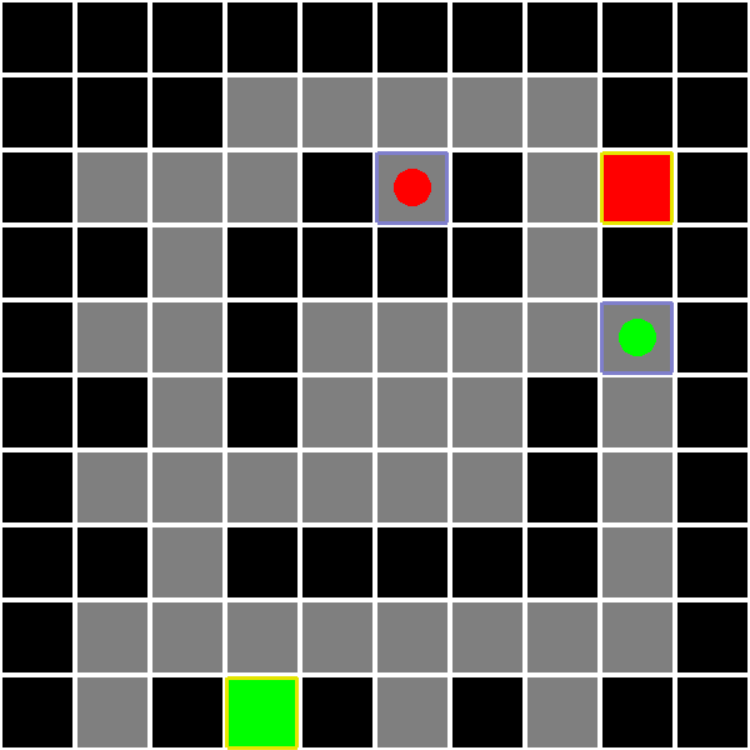
\includegraphics[width=0.8\textwidth]{picture/cooperative_navigation.png}  
     \end{minipage}
    }
    \subfigure[Predator and Prey] {
     \label{Predator and Prey env}
     \begin{minipage}[t]{0.3\linewidth}
     \centering 
     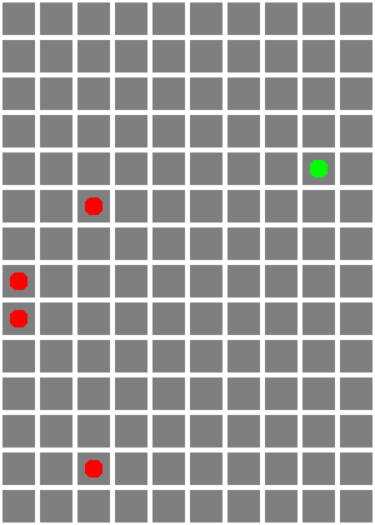
\includegraphics[width=0.7\textwidth]{picture/predator and prey.png}  
     \end{minipage}
    }
    \subfigure[Multi-Room Search] {
     \label{Multi-Room Search env}     
     \begin{minipage}[t]{0.3\linewidth}
     \centering
     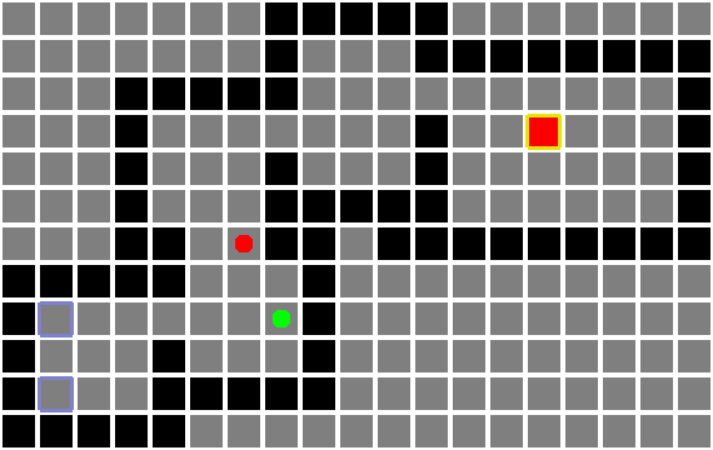
\includegraphics[width=1.1\textwidth]{picture/multi-room search.png}
     \end{minipage}
    } 
    \caption{Environment scenarios}
    \label{environment scenarios}
\end{figure}


\subsection{Cooperative Navigation}
In this scenario, two agent(red and green circles) must cooperatively collect all treasures(red and green squares) on the map in order to complete the task, at each time step, agents choose one of five actions: up, down, left, right or stay still, and move to adjacent grids according to the action if not blocked by walk(black grids) or other agents, a reward of 50 is award to each agent when all treasure are collected and agents receive a step penalty of 0.1 whenever take a step.
\begin{figure}
\centering
    \subfigure{
     \label{compare_env1}
     \begin{minipage}[t]{0.48\linewidth}
     \centering 
     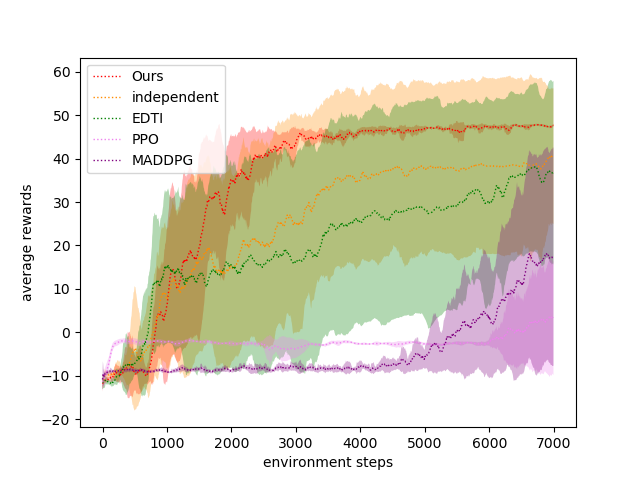
\includegraphics[width=1\textwidth]{picture/compare_env1.png}  
     \end{minipage}
    }
    \subfigure{
     \label{abu_env1}     
     \begin{minipage}[t]{0.48\linewidth}
     \centering
     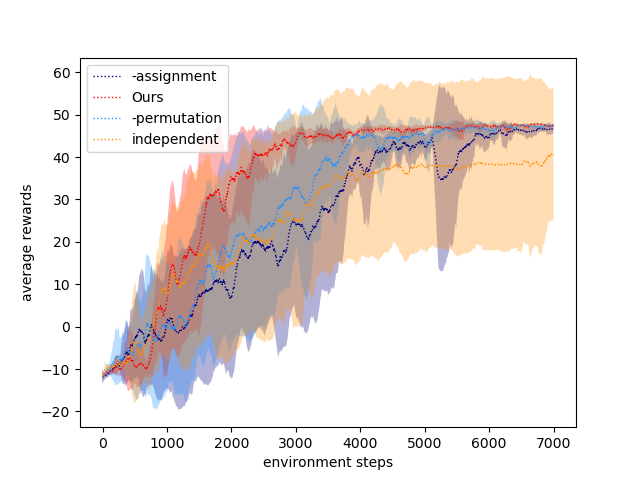
\includegraphics[width=1\textwidth]{picture/abu_env1.png}
     \end{minipage}
    } 
    \caption{Two agent are required to find the two treasures in the grid world. We plot the mean rewards of}
    \label{Cooperative Navigation}
\end{figure}

\subsection{Predator and Prey}
As shown in \ref{Predator and Prey env}, in this scenario four predator(red circles) aim to catch a prey(greed circle) cooperatively, predators spawn randomly on the bottom of the world, prey on the top. Prey moves randomly and is restricted its position to the top 5 rows, it's caught by the predators only if predators/boundaries surround it on all sides. An episode ends either when the prey is caught or after 100 steps, all predators received a reward of 20 when catching the prey.
\iffalse
\begin{figure}
\centering
    \subfigure {
     \label{compare_env2}
     \begin{minipage}[t]{0.48\linewidth}
     \centering 
     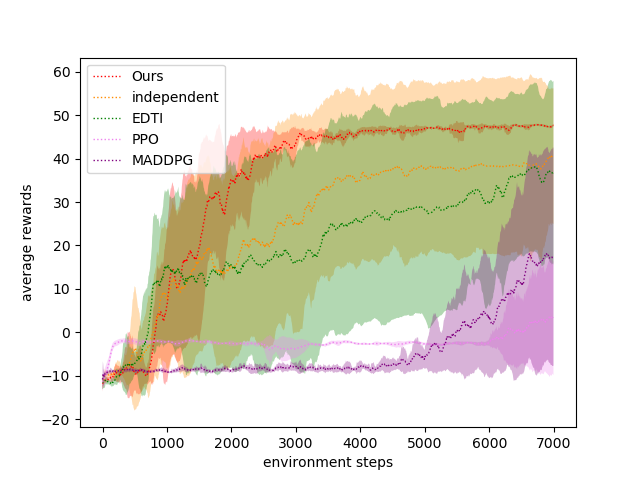
\includegraphics[width=1\textwidth]{picture/compare_env1.png}  
     \end{minipage}
    }
    \subfigure {
     \label{abu_env2}     
     \begin{minipage}[t]{0.48\linewidth}
     \centering
     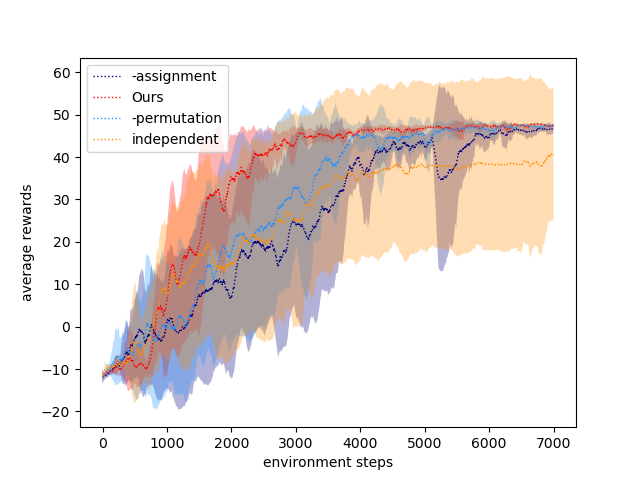
\includegraphics[width=1\textwidth]{picture/abu_env1.png}
     \end{minipage}
    } 
    \caption{Two agent are required to find the two treasures in the grid world. We plot the mean rewards of }
    \label{predator and prey}
\end{figure}
\fi
\subsection{Multi-Room Search}
In this scenario, agents(red and greed circles) must go through several doors to enter the final room to get the treasure(red square) together. The door connected two adjacent rooms always allows only one agent to pass through which need two agents to pass cooperatively.
\begin{figure}
\centering
    \subfigure{
     \label{compare_env3}
     \begin{minipage}[t]{0.48\linewidth}
     \centering 
     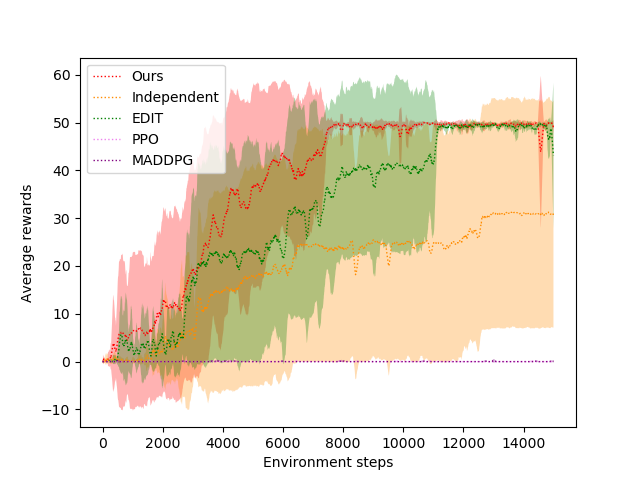
\includegraphics[width=1\textwidth]{picture/compare_env3.png}  
     \end{minipage}
    }
    \subfigure{
     \label{abu_env3}     
     \begin{minipage}[t]{0.48\linewidth}
     \centering
     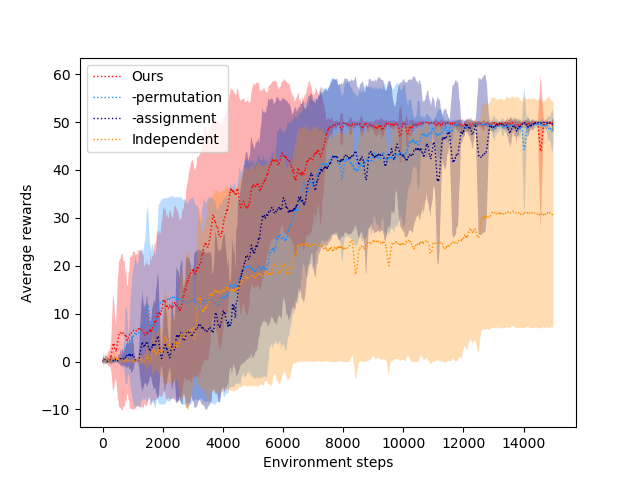
\includegraphics[width=1\textwidth]{picture/abu_env3.png}
     \end{minipage}
    } 
    \caption{Two agent are required to find the two treasures in the grid world. We plot the mean rewards of }
    \label{multi-Room search}
\end{figure}
\section{Conclusion}






\iffalse
\section{Submission of conference papers to ICLR 2021}

ICLR requires electronic submissions, processed by
\url{https://openreview.net/}. See ICLR's website for more instructions.

If your paper is ultimately accepted, the statement {\tt
  {\textbackslash}iclrfinalcopy} should be inserted to adjust the
format to the camera ready requirements.

The format for the submissions is a variant of the NeurIPS format.
Please read carefully the instructions below, and follow them
faithfully.

\subsection{Style}

Papers to be submitted to ICLR 2021 must be prepared according to the
instructions presented here.

%% Please note that we have introduced automatic line number generation
%% into the style file for \LaTeXe. This is to help reviewers
%% refer to specific lines of the paper when they make their comments. Please do
%% NOT refer to these line numbers in your paper as they will be removed from the
%% style file for the final version of accepted papers.

Authors are required to use the ICLR \LaTeX{} style files obtainable at the
ICLR website. Please make sure you use the current files and
not previous versions. Tweaking the style files may be grounds for rejection.

\subsection{Retrieval of style files}

The style files for ICLR and other conference information are available online at:
\begin{center}
   \url{http://www.iclr.cc/}
\end{center}
The file \verb+iclr2021_conference.pdf+ contains these
instructions and illustrates the
various formatting requirements your ICLR paper must satisfy.
Submissions must be made using \LaTeX{} and the style files
\verb+iclr2021_conference.sty+ and \verb+iclr2021_conference.bst+ (to be used with \LaTeX{}2e). The file
\verb+iclr2021_conference.tex+ may be used as a ``shell'' for writing your paper. All you
have to do is replace the author, title, abstract, and text of the paper with
your own.

The formatting instructions contained in these style files are summarized in
sections \ref{gen_inst}, \ref{headings}, and \ref{others} below.

\section{General formatting instructions}
\label{gen_inst}

The text must be confined within a rectangle 5.5~inches (33~picas) wide and
9~inches (54~picas) long. The left margin is 1.5~inch (9~picas).
Use 10~point type with a vertical spacing of 11~points. Times New Roman is the
preferred typeface throughout. Paragraphs are separated by 1/2~line space,
with no indentation.

Paper title is 17~point, in small caps and left-aligned.
All pages should start at 1~inch (6~picas) from the top of the page.

Authors' names are
set in boldface, and each name is placed above its corresponding
address. The lead author's name is to be listed first, and
the co-authors' names are set to follow. Authors sharing the
same address can be on the same line.

Please pay special attention to the instructions in section \ref{others}
regarding figures, tables, acknowledgments, and references.


There will be a strict upper limit of 8 pages for the main text of the initial submission, with unlimited additional pages for citations. Note that the upper page limit differs from last year!Authors may use as many pages of appendices (after the bibliography) as they wish, but reviewers are not required to read these. During the rebuttal phase and for the camera ready version, authors are allowed one additional page for the main text, for a strict upper limit of 9 pages.

\section{Headings: first level}
\label{headings}

First level headings are in small caps,
flush left and in point size 12. One line space before the first level
heading and 1/2~line space after the first level heading.

\subsection{Headings: second level}

Second level headings are in small caps,
flush left and in point size 10. One line space before the second level
heading and 1/2~line space after the second level heading.

\subsubsection{Headings: third level}

Third level headings are in small caps,
flush left and in point size 10. One line space before the third level
heading and 1/2~line space after the third level heading.

\section{Citations, figures, tables, references}
\label{others}

These instructions apply to everyone, regardless of the formatter being used.

\subsection{Citations within the text}

Citations within the text should be based on the \texttt{natbib} package
and include the authors' last names and year (with the ``et~al.'' construct
for more than two authors). When the authors or the publication are
included in the sentence, the citation should not be in parenthesis using \verb|\citet{}| (as
in ``See \citet{Hinton06} for more information.''). Otherwise, the citation
should be in parenthesis using \verb|\citep{}| (as in ``Deep learning shows promise to make progress
towards AI~\citep{Bengio+chapter2007}.'').

The corresponding references are to be listed in alphabetical order of
authors, in the \textsc{References} section. As to the format of the
references themselves, any style is acceptable as long as it is used
consistently.

\subsection{Footnotes}

Indicate footnotes with a number\footnote{Sample of the first footnote} in the
text. Place the footnotes at the bottom of the page on which they appear.
Precede the footnote with a horizontal rule of 2~inches
(12~picas).\footnote{Sample of the second footnote}

\subsection{Figures}

All artwork must be neat, clean, and legible. Lines should be dark
enough for purposes of reproduction; art work should not be
hand-drawn. The figure number and caption always appear after the
figure. Place one line space before the figure caption, and one line
space after the figure. The figure caption is lower case (except for
first word and proper nouns); figures are numbered consecutively.

Make sure the figure caption does not get separated from the figure.
Leave sufficient space to avoid splitting the figure and figure caption.

You may use color figures.
However, it is best for the
figure captions and the paper body to make sense if the paper is printed
either in black/white or in color.
\begin{figure}[h]
\begin{center}
%\framebox[4.0in]{$\;$}
\fbox{\rule[-.5cm]{0cm}{4cm} \rule[-.5cm]{4cm}{0cm}}
\end{center}
\caption{Sample figure caption.}
\end{figure}

\subsection{Tables}

All tables must be centered, neat, clean and legible. Do not use hand-drawn
tables. The table number and title always appear before the table. See
Table~\ref{sample-table}.

Place one line space before the table title, one line space after the table
title, and one line space after the table. The table title must be lower case
(except for first word and proper nouns); tables are numbered consecutively.

\begin{table}[t]
\caption{Sample table title}
\label{sample-table}
\begin{center}
\begin{tabular}{ll}
\multicolumn{1}{c}{\bf PART}  &\multicolumn{1}{c}{\bf DESCRIPTION}
\\ \hline \\
Dendrite         &Input terminal \\
Axon             &Output terminal \\
Soma             &Cell body (contains cell nucleus) \\
\end{tabular}
\end{center}
\end{table}

\section{Default Notation}

In an attempt to encourage standardized notation, we have included the
notation file from the textbook, \textit{Deep Learning}
\cite{goodfellow2016deep} available at
\url{https://github.com/goodfeli/dlbook_notation/}.  Use of this style
is not required and can be disabled by commenting out
\texttt{math\_commands.tex}.


\centerline{\bf Numbers and Arrays}
\bgroup
\def\arraystretch{1.5}
\begin{tabular}{p{1in}p{3.25in}}
$\displaystyle a$ & A scalar (integer or real)\\
$\displaystyle \va$ & A vector\\
$\displaystyle \mA$ & A matrix\\
$\displaystyle \tA$ & A tensor\\
$\displaystyle \mI_n$ & Identity matrix with $n$ rows and $n$ columns\\
$\displaystyle \mI$ & Identity matrix with dimensionality implied by context\\
$\displaystyle \ve^{(i)}$ & Standard basis vector $[0,\dots,0,1,0,\dots,0]$ with a 1 at position $i$\\
$\displaystyle \text{diag}(\va)$ & A square, diagonal matrix with diagonal entries given by $\va$\\
$\displaystyle \ra$ & A scalar random variable\\
$\displaystyle \rva$ & A vector-valued random variable\\
$\displaystyle \rmA$ & A matrix-valued random variable\\
\end{tabular}
\egroup
\vspace{0.25cm}

\centerline{\bf Sets and Graphs}
\bgroup
\def\arraystretch{1.5}

\begin{tabular}{p{1.25in}p{3.25in}}
$\displaystyle \sA$ & A set\\
$\displaystyle \R$ & The set of real numbers \\
$\displaystyle \{0, 1\}$ & The set containing 0 and 1 \\
$\displaystyle \{0, 1, \dots, n \}$ & The set of all integers between $0$ and $n$\\
$\displaystyle [a, b]$ & The real interval including $a$ and $b$\\
$\displaystyle (a, b]$ & The real interval excluding $a$ but including $b$\\
$\displaystyle \sA \backslash \sB$ & Set subtraction, i.e., the set containing the elements of $\sA$ that are not in $\sB$\\
$\displaystyle \gG$ & A graph\\
$\displaystyle \parents_\gG(\ervx_i)$ & The parents of $\ervx_i$ in $\gG$
\end{tabular}
\vspace{0.25cm}


\centerline{\bf Indexing}
\bgroup
\def\arraystretch{1.5}

\begin{tabular}{p{1.25in}p{3.25in}}
$\displaystyle \eva_i$ & Element $i$ of vector $\va$, with indexing starting at 1 \\
$\displaystyle \eva_{-i}$ & All elements of vector $\va$ except for element $i$ \\
$\displaystyle \emA_{i,j}$ & Element $i, j$ of matrix $\mA$ \\
$\displaystyle \mA_{i, :}$ & Row $i$ of matrix $\mA$ \\
$\displaystyle \mA_{:, i}$ & Column $i$ of matrix $\mA$ \\
$\displaystyle \etA_{i, j, k}$ & Element $(i, j, k)$ of a 3-D tensor $\tA$\\
$\displaystyle \tA_{:, :, i}$ & 2-D slice of a 3-D tensor\\
$\displaystyle \erva_i$ & Element $i$ of the random vector $\rva$ \\
\end{tabular}
\egroup
\vspace{0.25cm}


\centerline{\bf Calculus}
\bgroup
\def\arraystretch{1.5}
\begin{tabular}{p{1.25in}p{3.25in}}
% NOTE: the [2ex] on the next line adds extra height to that row of the table.
% Without that command, the fraction on the first line is too tall and collides
% with the fraction on the second line.
$\displaystyle\frac{d y} {d x}$ & Derivative of $y$ with respect to $x$\\ [2ex]
$\displaystyle \frac{\partial y} {\partial x} $ & Partial derivative of $y$ with respect to $x$ \\
$\displaystyle \nabla_\vx y $ & Gradient of $y$ with respect to $\vx$ \\
$\displaystyle \nabla_\mX y $ & Matrix derivatives of $y$ with respect to $\mX$ \\
$\displaystyle \nabla_\tX y $ & Tensor containing derivatives of $y$ with respect to $\tX$ \\
$\displaystyle \frac{\partial f}{\partial \vx} $ & Jacobian matrix $\mJ \in \R^{m\times n}$ of $f: \R^n \rightarrow \R^m$\\
$\displaystyle \nabla_\vx^2 f(\vx)\text{ or }\mH( f)(\vx)$ & The Hessian matrix of $f$ at input point $\vx$\\
$\displaystyle \int f(\vx) d\vx $ & Definite integral over the entire domain of $\vx$ \\
$\displaystyle \int_\sS f(\vx) d\vx$ & Definite integral with respect to $\vx$ over the set $\sS$ \\
\end{tabular}
\egroup
\vspace{0.25cm}

\centerline{\bf Probability and Information Theory}
\bgroup
\def\arraystretch{1.5}
\begin{tabular}{p{1.25in}p{3.25in}}
$\displaystyle P(\ra)$ & A probability distribution over a discrete variable\\
$\displaystyle p(\ra)$ & A probability distribution over a continuous variable, or over
a variable whose type has not been specified\\
$\displaystyle \ra \sim P$ & Random variable $\ra$ has distribution $P$\\% so thing on left of \sim should always be a random variable, with name beginning with \r
$\displaystyle  \E_{\rx\sim P} [ f(x) ]\text{ or } \E f(x)$ & Expectation of $f(x)$ with respect to $P(\rx)$ \\
$\displaystyle \Var(f(x)) $ &  Variance of $f(x)$ under $P(\rx)$ \\
$\displaystyle \Cov(f(x),g(x)) $ & Covariance of $f(x)$ and $g(x)$ under $P(\rx)$\\
$\displaystyle H(\rx) $ & Shannon entropy of the random variable $\rx$\\
$\displaystyle \KL ( P \Vert Q ) $ & Kullback-Leibler divergence of P and Q \\
$\displaystyle \mathcal{N} ( \vx ; \vmu , \mSigma)$ & Gaussian distribution %
over $\vx$ with mean $\vmu$ and covariance $\mSigma$ \\
\end{tabular}
\egroup
\vspace{0.25cm}

\centerline{\bf Functions}
\bgroup
\def\arraystretch{1.5}
\begin{tabular}{p{1.25in}p{3.25in}}
$\displaystyle f: \sA \rightarrow \sB$ & The function $f$ with domain $\sA$ and range $\sB$\\
$\displaystyle f \circ g $ & Composition of the functions $f$ and $g$ \\
  $\displaystyle f(\vx ; \vtheta) $ & A function of $\vx$ parametrized by $\vtheta$.
  (Sometimes we write $f(\vx)$ and omit the argument $\vtheta$ to lighten notation) \\
$\displaystyle \log x$ & Natural logarithm of $x$ \\
$\displaystyle \sigma(x)$ & Logistic sigmoid, $\displaystyle \frac{1} {1 + \exp(-x)}$ \\
$\displaystyle \zeta(x)$ & Softplus, $\log(1 + \exp(x))$ \\
$\displaystyle || \vx ||_p $ & $\normlp$ norm of $\vx$ \\
$\displaystyle || \vx || $ & $\normltwo$ norm of $\vx$ \\
$\displaystyle x^+$ & Positive part of $x$, i.e., $\max(0,x)$\\
$\displaystyle \1_\mathrm{condition}$ & is 1 if the condition is true, 0 otherwise\\
\end{tabular}
\egroup
\vspace{0.25cm}



\section{Final instructions}
Do not change any aspects of the formatting parameters in the style files.
In particular, do not modify the width or length of the rectangle the text
should fit into, and do not change font sizes (except perhaps in the
\textsc{References} section; see below). Please note that pages should be
numbered.

\section{Preparing PostScript or PDF files}

Please prepare PostScript or PDF files with paper size ``US Letter'', and
not, for example, ``A4''. The -t
letter option on dvips will produce US Letter files.

Consider directly generating PDF files using \verb+pdflatex+
(especially if you are a MiKTeX user).
PDF figures must be substituted for EPS figures, however.

Otherwise, please generate your PostScript and PDF files with the following commands:
\begin{verbatim}
dvips mypaper.dvi -t letter -Ppdf -G0 -o mypaper.ps
ps2pdf mypaper.ps mypaper.pdf
\end{verbatim}

\subsection{Margins in LaTeX}

Most of the margin problems come from figures positioned by hand using
\verb+\special+ or other commands. We suggest using the command
\verb+\includegraphics+
from the graphicx package. Always specify the figure width as a multiple of
the line width as in the example below using .eps graphics
\begin{verbatim}
   \usepackage[dvips]{graphicx} ...
   \includegraphics[width=0.8\linewidth]{myfile.eps}
\end{verbatim}
or % Apr 2009 addition
\begin{verbatim}
   \usepackage[pdftex]{graphicx} ...
   \includegraphics[width=0.8\linewidth]{myfile.pdf}
\end{verbatim}
for .pdf graphics.
See section~4.4 in the graphics bundle documentation (\url{http://www.ctan.org/tex-archive/macros/latex/required/graphics/grfguide.ps})

A number of width problems arise when LaTeX cannot properly hyphenate a
line. Please give LaTeX hyphenation hints using the \verb+\-+ command.

\subsubsection*{Author Contributions}
If you'd like to, you may include  a section for author contributions as is done
in many journals. This is optional and at the discretion of the authors.

\subsubsection*{Acknowledgments}
Use unnumbered third level headings for the acknowledgments. All
acknowledgments, including those to funding agencies, go at the end of the paper.
\fi


\bibliography{iclr2021_conference}
\bibliographystyle{iclr2021_conference}

\appendix
\section{Appendix}
You may include other additional sections here.

\end{document}
